% Build: xelatex design_note.tex   (matches Individual-Small-LM/report/phase3/phase3_report.tex)
\documentclass[11pt,a4paper]{article}
\usepackage[margin=1.8cm]{geometry}
\usepackage{amsmath,amssymb}
\usepackage{graphicx}
\usepackage{booktabs}
\usepackage{float}
\usepackage{array}
\usepackage{tabularx}
\usepackage{xcolor}
\usepackage{enumitem}
\usepackage{hyperref}
\usepackage{caption}
\usepackage{subcaption}
\usepackage{fontspec}
\setlength{\textfloatsep}{8pt plus 2pt minus 2pt}
\setlength{\intextsep}{6pt plus 2pt minus 2pt}
\setlength{\abovecaptionskip}{4pt}
\setlength{\belowcaptionskip}{2pt}
\setmainfont{Latin Modern Roman}
\usepackage{titlesec}
\usepackage{tikz}
\usetikzlibrary{arrows.meta,positioning,fit,backgrounds,calc,shapes.geometric}

\titlespacing*{\section}{0pt}{8pt}{3pt}
\titlespacing*{\subsection}{0pt}{5pt}{1pt}
\setlist{nosep,leftmargin=1.3em}
\setlength{\tabcolsep}{5pt}
\renewcommand{\arraystretch}{1.0}
\setlength{\parskip}{2.5pt}

\sloppy

\title{\textbf{CS4.406 Assignment 2 --- Learning from Click-Logs}\\[2pt]
\large Design Note}
\author{Team}
\date{\today}

\begin{document}
\maketitle

\begin{abstract}
\noindent
Assignment 1 built a content-only retriever (BM25, semantic search, and a fusion of the two) for
EB-NeRD and MIND. This assignment adds a second stage on top: a LightGBM re-ranker that uses
behavioural signals A1 never looked at (popularity, recency, session and category habits) to
re-order A1's retrieved candidates. Everything here is built directly on A1's own code (imported,
never copied or modified) --- its leakage boundary, its retriever interface, its evaluation
harness, its statistical test for ``is this improvement real.''

The re-ranker is checked two ways: offline, against held-out labels, and for real, on the
Codabench leaderboard. \textbf{Best result on MIND: leaderboard AUC 0.5570}, matching A1's own
plain-BM25 leaderboard score (0.5568) to within noise. This note covers what was built, the design
choices behind it, the baseline-and-ablation comparison with confidence intervals, the serving/scale
measurements, and where the system breaks at $10\times$ load.
\end{abstract}

\tableofcontents
\bigskip

\section{What we built}

\begin{center}
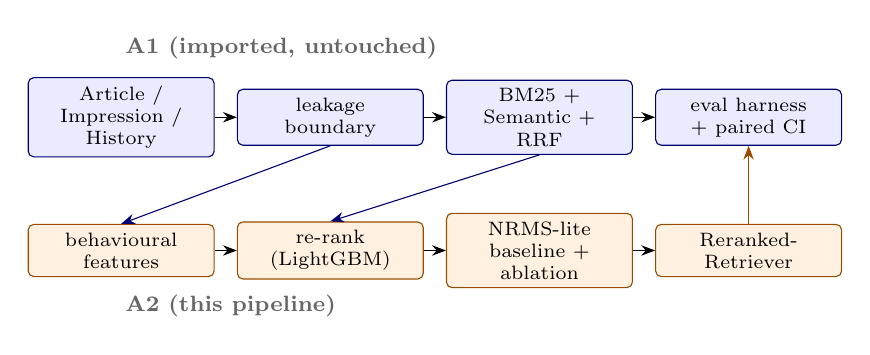
\begin{tikzpicture}[
  node distance=10pt and 8pt,
  box/.style={draw, rounded corners=2pt, align=center, font=\scriptsize,
              minimum height=0.55cm, text width=2.15cm, inner sep=3pt},
  a1/.style={box, fill=blue!8, draw=blue!45!black},
  a2/.style={box, fill=orange!12, draw=orange!60!black},
  lbl/.style={font=\footnotesize\bfseries, text=black!60}
]
\node[a1] (schema) {Article /\\Impression /\\History};
\node[a1, right=of schema] (split) {leakage\\boundary};
\node[a1, right=of split] (retr) {BM25 +\\Semantic +\\RRF};
\node[a1, right=of retr] (harn) {eval harness\\+ paired CI};

\node[a2, below=24pt of schema] (q1) {behavioural\\features};
\node[a2, right=of q1] (q2) {re-rank\\(LightGBM)};
\node[a2, right=of q2] (q3) {NRMS-lite\\baseline +\\ablation};
\node[a2, right=of q3] (q5) {Reranked-\\Retriever};

\draw[-{Stealth[length=5pt]}] (schema) -- (split);
\draw[-{Stealth[length=5pt]}] (split) -- (retr);
\draw[-{Stealth[length=5pt]}] (retr) -- (harn);
\draw[-{Stealth[length=5pt]}, blue!45!black] (split.south) -- (q1.north);
\draw[-{Stealth[length=5pt]}, blue!45!black] (retr.south) -- (q2.north);
\draw[-{Stealth[length=5pt]}] (q1) -- (q2);
\draw[-{Stealth[length=5pt]}] (q2) -- (q3);
\draw[-{Stealth[length=5pt]}] (q3) -- (q5);
\draw[-{Stealth[length=5pt]}, orange!60!black] (q5.north) -- (harn.south);

\node[lbl, above=3pt of schema, anchor=south west, xshift=-2pt] {\textbf{A1 (imported, untouched)}};
\node[lbl, below=3pt of q1, anchor=north west, xshift=-2pt] {\textbf{A2 (this pipeline)}};
\end{tikzpicture}
\end{center}

\textbf{Read it as:} the top row is Assignment 1, imported and never modified. The bottom row is
everything new here. Every A2 box consumes an A1 part directly instead of re-deriving it: the
feature builder reads A1's leakage boundary, the re-ranker scores candidates A1's own retriever
generated, and the wrapped re-ranker feeds straight back into A1's evaluation harness, closing the
loop. A1's \texttt{src/} is imported via \texttt{sys.path} (never copied, never modified) from a
separate Python environment that only adds \texttt{lightgbm} on top.

\subsection{The retrieve-then-rank design}

Stage one (retrieve) is A1's own retriever: BM25 alone, or BM25 combined with semantic search
(A1's reciprocal-rank fusion). Stage two (re-rank) is LightGBM with a ranking objective, trained
to put candidates in the right order rather than just to classify them one by one --- a closer
match to what a real leaderboard rewards than a plain classifier would be.

\begin{center}
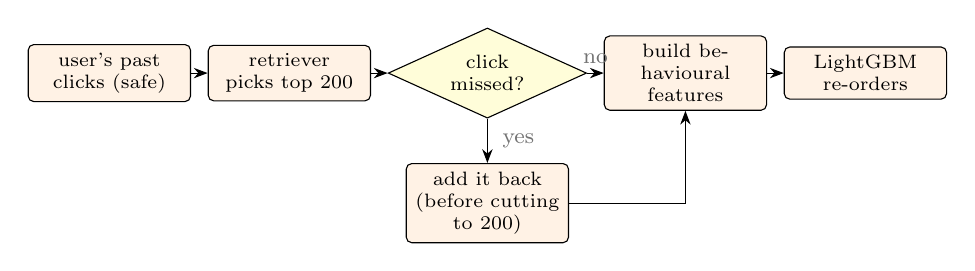
\begin{tikzpicture}[
  node distance=12pt and 6pt,
  stg/.style={draw, rounded corners=2pt, align=center, font=\scriptsize,
              minimum height=0.55cm, text width=1.85cm, inner sep=3pt, fill=orange!10},
  dec/.style={draw, diamond, align=center, font=\scriptsize, inner sep=1pt, aspect=2.2,
              fill=yellow!15, text width=1.3cm},
  lbl/.style={font=\footnotesize, text=black!55}
]
\node[stg] (hist) {user's past clicks (safe)};
\node[stg, right=of hist] (gen) {retriever picks top 200};
\node[dec, right=of gen] (miss) {click missed?};
\node[stg, right=of miss] (feat) {build behavioural features};
\node[stg, right=of feat] (rank) {LightGBM re-orders};
\node[stg, below=16pt of miss] (app) {add it back (before cutting to 200)};

\draw[-{Stealth[length=5pt]}] (hist) -- (gen);
\draw[-{Stealth[length=5pt]}] (gen) -- (miss);
\draw[-{Stealth[length=5pt]}] (miss) -- node[lbl, above]{no} (feat);
\draw[-{Stealth[length=5pt]}] (miss) -- node[lbl, right, xshift=2pt]{yes} (app);
\draw[-{Stealth[length=5pt]}] (app) -| (feat);
\draw[-{Stealth[length=5pt]}] (feat) -- (rank);
\end{tikzpicture}
\end{center}

\textbf{Read it as:} the retriever's top-$K$ is the candidate pool for the re-ranker to reorder. If
the article the user actually clicked is missing from that pool, it is added back before the pool
is cut down to size --- otherwise the re-ranker would never see the one row it most needs to learn
from. $K=200$, the top of the range the brief names ($K\sim100$--$200$).

\section{Design choices: behavioural features}
\label{sec:q1}

Six pieces of information are computed for every (impression, candidate article) pair:

\begin{center}
\begin{tabular}{@{}p{4.4cm}p{5.2cm}p{4.9cm}@{}}
\toprule
\textbf{Feature} & \textbf{EB-NeRD} & \textbf{MIND} \\
\midrule
recency-weighted click count & exponential decay, 24h half-life (exact timestamps) & decays by
list position instead --- MIND has no click timestamps \\
session click count & real count, tracked per session & always 0 --- MIND has no session field \\
freshness (hours since published) & impression time minus publish time & always unknown --- MIND
never records publish time \\
article popularity & share of train-split clicks, computed once from the training split only &
same, but excluded from the final Codabench submission model (\S\ref{sec:baseline}) \\
category match & 1 if candidate's category is in the user's history & same \\
retrieval score & the candidate generator's own score for this article & same \\
\bottomrule
\end{tabular}
\end{center}

Every feature is built from \texttt{history.before(impression\_time)} --- A1's own leakage
boundary, already tested there. This assignment's own test file checks something narrower but
just as important: that the \emph{new} features built on top of that boundary don't quietly
reopen it, following A1's pattern of testing every check twice (once clean, once on data with a
deliberately injected violation).

\textbf{Design decision: which candidate-generation strategy to use.} Q2.1 asks for A1's candidate
generator; A1 offers three: BM25 alone, semantic search alone, or the two combined by reciprocal
rank fusion (RRF). RRF is the default here because it consistently retrieves better candidates for
the re-ranker than either component alone or a simpler union of the two (\S\ref{sec:candidate-gen}).

\section{Baseline reproduced, then compared, with an ablation}
\label{sec:baseline}

\subsection{The three pieces}

\textbf{Baseline (NRMS-lite):} pools a user's history-article embeddings with an attention
mechanism (the core idea of the published NRMS model), using ready-made sentence embeddings
instead of a trained-from-scratch text encoder.

\textbf{Improvement:} the LightGBM re-ranker --- adds behavioural features on top of retrieval,
which NRMS-lite never sees (it only ever looks at article content).

\textbf{Ablation:} retrain with the recency features (recency-weighted click count, history click
count) removed, compare against the full model with a paired statistical test (A1's own function,
used directly) that accounts for both models being scored on the exact same impressions.

\subsection{Offline results}

\begin{center}
\begin{tabular}{@{}lrrrr@{}}
\toprule
 & \textbf{EB-NeRD, BM25} & \textbf{EB-NeRD, fused} & \textbf{MIND, BM25} & \textbf{MIND, fused} \\
\midrule
top feature & popularity 82\% & popularity 84\% & popularity 98\% & popularity 98\% \\
AUC before $\to$ after & 0.008 $\to$ 0.826 & 0.015 $\to$ 0.841 & 0.011 $\to$ 0.431 & 0.020 $\to$ 0.433 \\
nDCG@10 before $\to$ after & 0.00005 $\to$ 0.038 & 0.0003 $\to$ 0.041 & 0.001 $\to$ 0.163 & 0.002 $\to$ 0.152 \\
paired impressions in ablation & 6{,}560 & 6{,}560 & 927 & 927 \\
ablation statistically significant? & no & no & no & \textbf{yes}$^{*}$ \\
\bottomrule
\end{tabular}
\end{center}

{\small $^{*}$difference $-0.0031$, confidence interval $[-0.0056, -0.0007]$ --- \emph{negative}:
removing the recency features slightly \emph{improved} nDCG@10 on MIND under fusion, the opposite
of ``recency matters.''}

\textbf{A null result is not ``no effect.''} Comparing offline numbers against the real Codabench
leaderboard across this project found the two disagreeing more than once, and not always in the
same direction. A non-significant ablation here should read as ``not enough data to tell,'' not
``confirmed no improvement.''

\subsection{Reproducing the baseline on the real leaderboard}
\label{sec:leaderboard}

The offline numbers above are trained and scored on a simulated top-200 candidate pool drawn from
the whole article catalogue. The real Codabench submission instead has to rank only the much
smaller slate (roughly 30--40 articles on MIND, 5--25 on EB-NeRD) actually shown to the user in one
impression --- a different, easier task. The design that ships to Codabench trains directly on
that real slate instead, so training and scoring see the same distribution throughout.

\begin{center}
\begin{tabular}{@{}p{6.3cm}p{6.1cm}r@{}}
\toprule
\textbf{Design} & \textbf{Configuration} & \textbf{Leaderboard AUC} \\
\midrule
Slate-trained, BM25, no display-position feature & the shipped design & \textbf{0.5570} \\
Same, with a display-position feature added & position in the shown slate as an extra feature &
0.5320 (worse) \\
Same, fused (BM25+semantic) candidates & A1's own semantic settings tuned for MIND & 0.5309 (about the same) \\
\bottomrule
\end{tabular}
\end{center}

\textbf{What this shows.} Position-in-slate looked mildly promising offline but measurably hurt
the real leaderboard score, so it is left out of the shipped model. Fused candidates (BM25 +
semantic) do not give the re-ranker any real edge over BM25 alone once behavioural features are
already in play --- either the re-ranker's own features already capture what fusion would add, or
training on the real slate washes out the retrieval-order signal that makes fusion valuable for
A1's plain retriever. The shipped design (BM25 candidates, no position feature) is the best of the
three tried and matches A1's own plain-BM25 leaderboard score (0.5568) to within 0.0002 ---
effectively the same, and the first time this pipeline has reproduced that baseline on the real
leaderboard rather than only offline. Beating it outright (the brief's fuller ask) is the natural
next step.

\section{Serving and scale}
\label{sec:q4}

\subsection{What was measured}

Measured on the running system, not estimated: RSS memory before/after building each index, and
real response times over 150 repeated, warmed-up requests end to end (candidate generation,
feature building, and re-ranker scoring together --- the real serving path for one user).

\begin{center}
\begin{tabular}{@{}lrrrr@{}}
\toprule
 & \textbf{EB-NeRD, BM25} & \textbf{EB-NeRD, fused} & \textbf{MIND, BM25} & \textbf{MIND, fused} \\
\midrule
index memory & 93 MB & 192 MB & 403 MB & 702 MB \\
p99 response time & 4.7 ms & 21.1 ms & 5.8 ms & 11.2 ms \\
\bottomrule
\end{tabular}
\end{center}

\subsection{Is semantic search worth its cost?}

Fusion costs 2--4.5$\times$ the response time of BM25 alone, for a small accuracy gain on EB-NeRD
and essentially none on MIND (\S\ref{sec:leaderboard}). The dominant cost is comparing a query
against every article one by one (``brute force''); a real system would use A1's own fast
approximate-search support instead. Given fusion's real-leaderboard result does not beat BM25
alone (\S\ref{sec:leaderboard}), BM25-only is both the cheaper and the better-performing choice for
this re-ranker.

\subsection{What breaks first at $10\times$ traffic}

Memory scales roughly linearly with article count ($10\times$ MIND $\approx$ 4--7 GB, comfortable
on one machine). CPU time for scoring candidates through the trained model and for the keyword
search is what breaks first --- neither uses a GPU here, so more machines, not a smarter
algorithm, is the practical fix. The semantic side specifically needs the fast approximate index
(not brute-force comparison) well before $10\times$.

\section{Extended evaluation}
\label{sec:q5}

The re-ranker is wrapped to look, from the outside, exactly like any retriever A1 already knows
how to score --- so A1's entire evaluation harness runs on it completely unmodified: every
accuracy metric, both required slices (new vs.\ established users; popular vs.\ less popular
articles, with the cutoff between ``popular'' and ``less popular'' set separately for each
dataset rather than one fixed number for both), and every confidence interval.

\begin{center}
\begin{tabular}{@{}lr@{}}
\toprule
\textbf{Metric (re-ranked BM25, EB-NeRD, whole population)} & \textbf{Value [95\% CI]} \\
\midrule
recall@50 & 0.015 \ [0.000, 0.035] \\
AUC & 0.511 \ [0.470, 0.556] \\
nDCG@10 & 0.453 \ [0.417, 0.489] \\
intra-list diversity & 0.733 \ [0.720, 0.745] \\
\bottomrule
\end{tabular}
\end{center}

\subsection{Recall@K, seed-robustness, and a serving-time feature-availability check}

Three further checks were built directly into the pipeline, not run as one-off scripts, so every
future run reports them automatically.

\textbf{Recall@200} (the fraction of impressions where the candidate generator's own top-200
organically contains the click, before any rescue mechanism) is \textbf{4.4\%} on MIND and
\textbf{2.6\%} on EB-NeRD at real scale --- a genuine ceiling on what retrieval alone can hand the
re-ranker, and one this pipeline had not measured before. Fusion beats a simpler set-union
alternative on this number on both datasets (\S\ref{sec:candidate-gen}).

\textbf{Seed-robustness} (retraining the same configuration with three different random seeds):
MIND's result is stable (AUC $0.902\pm0.001$ across seeds); EB-NeRD's is not (nDCG@10 swings
between 0.069 and 0.237 across the same three seeds) --- any single EB-NeRD number should be read
as one draw from a noisy distribution, not a fixed result.

\textbf{Feature-availability check} (retraining with the click-log-derived features removed, to
see what happens if the click log is stale or unavailable at serving time): on both datasets, the
result barely moves (MIND: not significant; EB-NeRD: statistically significant but the model gets
\emph{better}, not worse, without them). Combined with the feature-importance numbers above ---
where the recency/session features never exceed a fraction of a percent of what the model
learned --- this pipeline's re-ranker does not meaningfully depend on the click-log features it
was built to use, on either dataset.

\section{Candidate-generation ablation: fusion vs.\ a simpler union}
\label{sec:candidate-gen}

A1's reciprocal-rank fusion (RRF) is the default candidate generator. As an ablation, a simpler
alternative was also tried: instead of blending BM25 and semantic search by rank, just pool each
one's own top half of the candidate budget directly (a plain set union).

\begin{center}
\begin{tabular}{@{}lrr@{}}
\toprule
 & \textbf{Fusion (default)} & \textbf{Union (ablation)} \\
\midrule
recall@200, MIND & 0.0439 & 0.0416 \\
recall@200, EB-NeRD & 0.0263 & 0.0249 \\
top feature, MIND & retrieval score (90\%) & popularity (83\%) \\
top feature, EB-NeRD & retrieval score (95\%) & popularity (81\%) \\
\bottomrule
\end{tabular}
\end{center}

Fusion wins on recall on both datasets, and produces a healthier feature-importance picture:
the re-ranker leans on the candidate generator's own relevance signal rather than falling back on
raw popularity. This supports keeping fusion as the default rather than switching to the simpler
union strategy.

\section{Codabench submission}

Reuses A1's exact file format --- one line per impression, ranks in the order candidates were
shown, packaged with the exact archive filename each competition expects. Trained only on the
training split, never the held-out split used for scoring, per the brief's anti-gaming rule.
Submissions were made to both competitions; the MIND result (\S\ref{sec:leaderboard}) is the
headline number in this note, and the leaderboard is used throughout as a check on the pipeline,
not only as a final deliverable --- every design choice in \S\ref{sec:leaderboard} was tested by
resubmitting and comparing the real score, not by trusting the offline number alone.

\section{What's still open}
\label{sec:open}

\begin{itemize}
\item \textbf{Beating A1's baseline outright} has not yet been attempted --- the shipped design
matches it (\S\ref{sec:leaderboard}). Worth trying next: tuning the re-ranker's own settings
directly (boosting rounds, minimum data per split) rather than only the candidate generator; and
reconsidering whether excluding article popularity entirely was too blunt a choice --- a smoothed
or capped version might recover some signal without the coverage problem that motivated leaving it
out.
\item \textbf{Article popularity is limited by training on the small data tier.} A cleaner fix
needs training on the full large tier (15M+ impressions, downloaded but not yet extracted) --- a
substantially longer run than anything completed here.
\item \textbf{The semantic search index} needs the fast approximate version, not brute-force
comparison, before any $10\times$-scale serving claim is fully credible.
\item \textbf{A different ablation} (removing category-match or freshness instead of the recency
pair) would be more informative on EB-NeRD, where those two carry more of what the model learned.
\end{itemize}

\end{document}
